\vspace{-0.12in}
\section{Evaluation}
\vspace{-0.05in}
To validate our method, we focus on pick-and-place motions---a canonical industrial robotics requirement where super-nominal payload manipulation can significantly extend the operational envelope of robot arms while obeying strict hardware limits.\footnote{Please refer to the supplementary material for more details on compute hardware, problem domain, experimental setup, and baseline methods. Videos are available here: \url{https://payload-diffusion.github.io/}}
In our experiments, payloads were rigidly attached to the end-effector with a geometrically centered and uniform mass distribution. This was a deliberate experimental choice necessitated by the limited grasping force of our parallel gripper, ensuring repeatable execution across trials. Importantly, this choice is not a fundamental limitation of our method: as shown in the supplementary video, our approach is capable of handling non-rigidly attached objects and payloads with modest center-of-mass offsets, though some failure modes at higher payloads are also highlighted and explained there.
During execution, invalid trajectories generated by the diffusion model are simply not executed. For valid trajectories that fail due to unmodeled dynamics (e.g., payload oscillations), standard robot safety stops are triggered automatically. Our approach relies on the manufacturer's joint velocity controller for trajectory tracking, which provides sufficiently accurate state tracking for the tasks evaluated in this work.

\subsection{Comparison of Payload Encodings}

Our evaluation of different payload encodings, conducted with FiLM conditioning and payload encoding normalization, reveals several key insights in terms of planning success rate (\Cref{fig:bar}).
\begin{wrapfigure}{r}{0.6\textwidth}   % l or r = left / right, width = ~½ line
  \vspace{-1.2\baselineskip}            % tighten top gap (optional)
% \begin{figure}
  \centering
    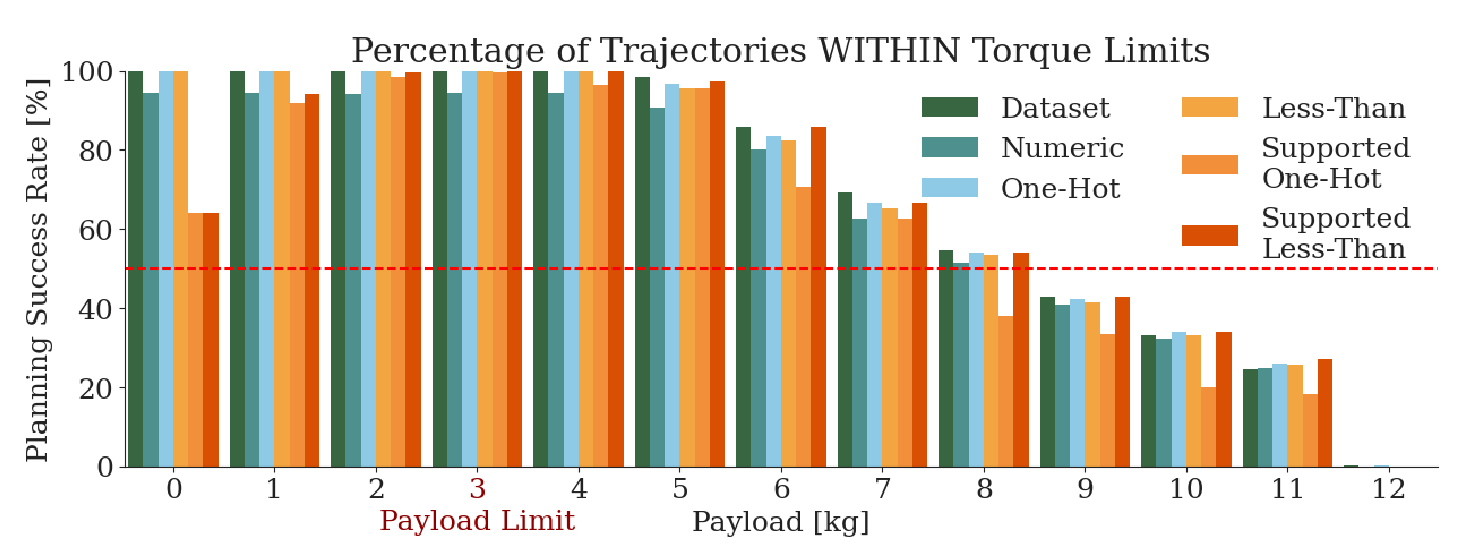
\includegraphics[width=\linewidth]{graphics/bar.pdf}
  \caption{The aggregate success rate metric shows one-hot diffusion closely matching the underlying training data distribution.}\label{fig:bar}
  \vspace{-1.3\baselineskip}            % tighten bottom gap (optional)
\end{wrapfigure}
Numeric and one-hot approaches demonstrate comparable effectiveness, particularly for payloads within nominal capacity ($0-3$kg). However, all methods show a tendency to underestimate success rates for higher payloads, potentially due to data imbalance in the training set. When interpreted as a less-than encoding during inference, the supported-range encoding achieves competitive performance, but its one-hot interpretation leads to significantly lower success rates.
While the encoding is designed to capture richer payload-trajectory relationships, the network struggles to fully utilize this information during generation.
The inability of numeric, supported one-hot, and supported less-than encodings to achieve $100\%$ success rates in the most loosely-constrained and data-rich portions of the state space, i.e., the nominal operating regime ($0-3$ kg), suggest fundamental limitations in how these encoding schemes enable the diffusion model to obey kinematic and dynamic constraints.
For subsequent experiments, we use with the one-hot encoding scheme, which demonstrates superior performance in terms of success rate.

\begin{figure}
  \centering
    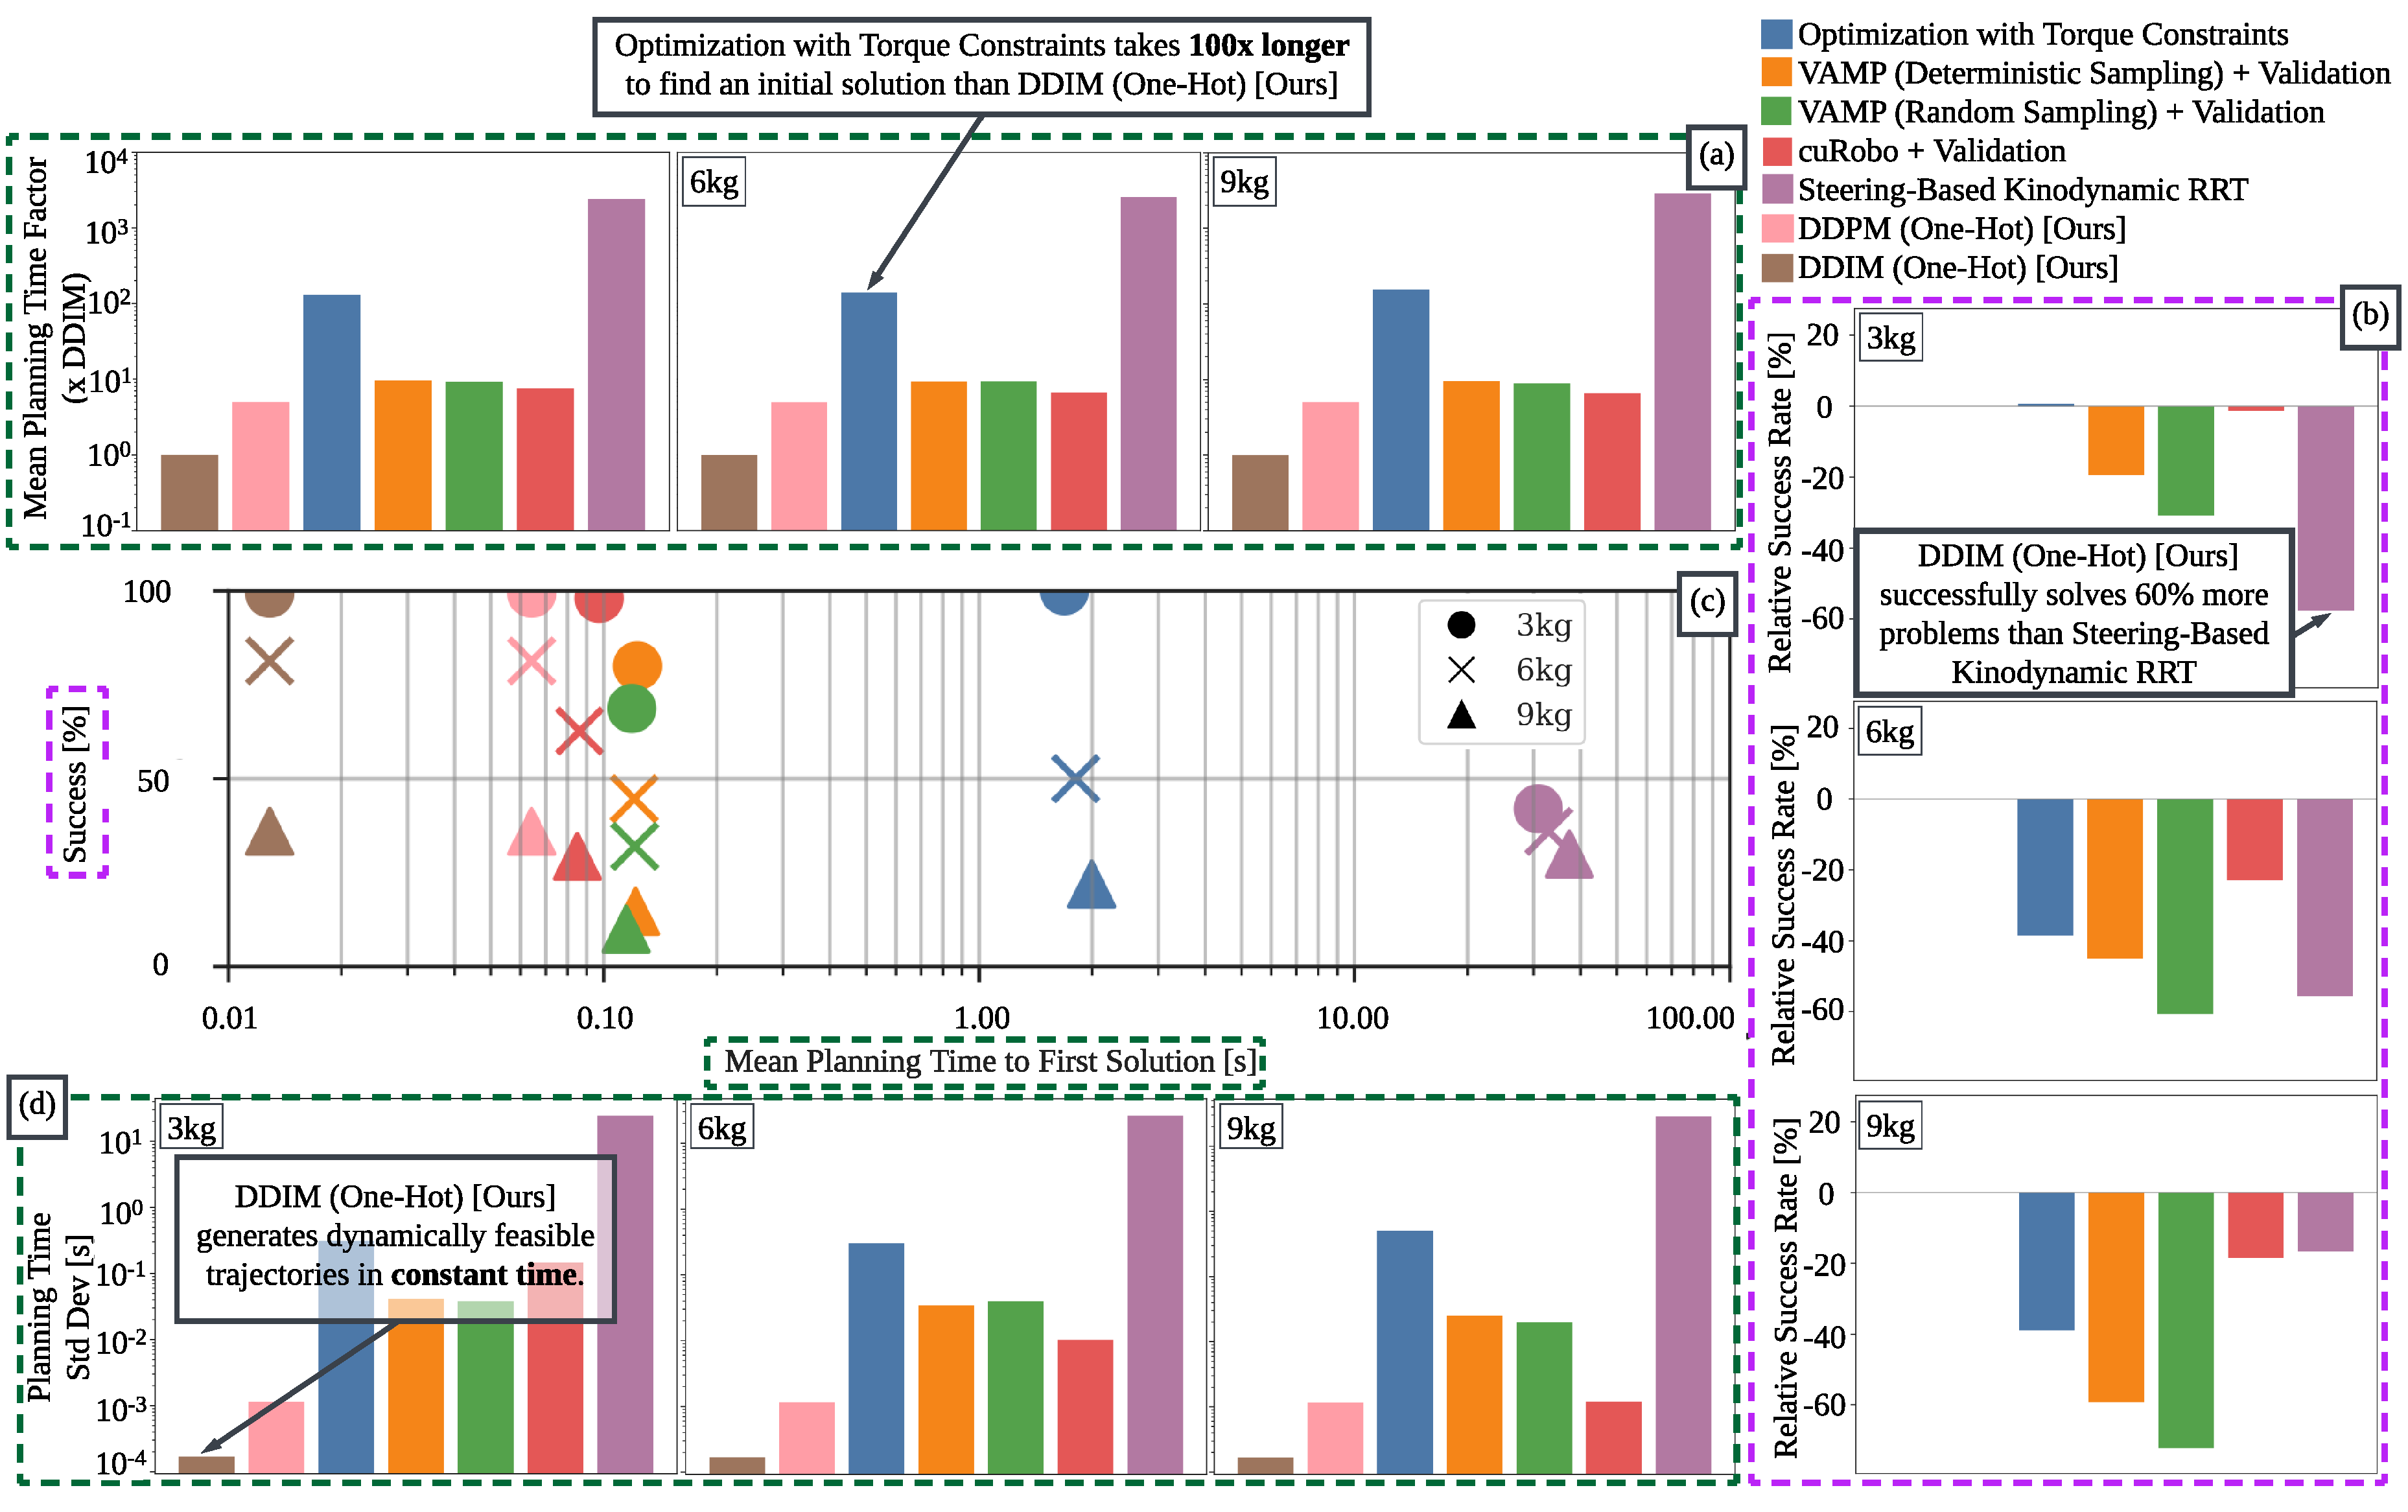
\includegraphics[width=\columnwidth]{graphics/eval.pdf}
  \caption{Comparative analysis of trajectory planning methods for payloads of $3$kg, $6$kg, and $9$kg. DDIM (One-Hot) significantly outperforms a variety of baseline methods in both planning time to first solution and success rate, generating dynamically feasible trajectories in constant time across all payload conditions.\vspace{-0.2in}}\label{fig:eval}
\end{figure}


\subsection{Comparison across Planner Types}

For the purposes of our discussion, we refer to DDIM (One-Hot) as a primary point of comparison. Denoising Diffusion Implicit Models (DDIM) offer accelerated inference due to fewer denoising steps (in our case, $5$) \cite{song2021denoising}. We also present results for DDPM \cite{ho2020denoising} with $25$ denoising steps. Notably, our experiments demonstrate that DDIM achieves identical success rates to DDPM despite requiring significantly less planning time ($\approx 0.01$s), validating our approach for realtime use (\Cref{fig:eval}c).

We evaluate our approach against a diverse set of trajectory planning methods using mean planning time to first solution and the corresponding success rate over $500$ tabletop manipulation tasks as the primary metric (\Cref{fig:eval}c). This metric provides a fair basis for comparison across fundamentally different planning paradigms. Additional metrics include planning time factor (mean planning time of baseline / mean planning time of DDIM) (\Cref{fig:eval}a), relative success rate change over DDIM as a percentage (\Cref{fig:eval}b), and standard deviations of planning times (\Cref{fig:eval}d). 

\paragraph{Plan-and-Filter Methods}

Broadly, plan-and-filter methods employ a sequential process: first planning a geometric path via sampling-based motion planning, then time-parameterizing it to derive joint velocities and accelerations, and finally validating trajectory feasibility for the target payload using the robot dynamics model (\cref{eq:arm-dyns}).
This iterative process continues until a feasible trajectory is found that satisfies all joint torque constraints induced by the payload \cite{abderezaei2024clutter}.
We evaluate two CPU-accelerated geometric planning variants: VAMP (RRTConnect) with deterministic sampling and VAMP (RRTConnect) with random sampling \cite{thomason2024motions}. We select Ruckig for time parameterization due to its ability to generate time-optimal trajectories in realtime \cite{berscheid2021jerk}.
Geometric motion planning and time parameterization can alternatively be unified within a single optimization framework (in our case, cuRobo) which can be followed by the dynamics validity checking.

Since there is a decoupling between kinematic reasoning and dynamic reasoning, further exacerbated by the separate time parameterization step in the VAMP variants, these approaches demonstrate inferior performance compared to our one-hot DDIM model (Fig. \ref{fig:eval}c).
VAMP with deterministic sampling achieves marginally higher success rates than VAMP with random sampling due to its low-dispersion sampling strategy, which provides more uniform exploration of the configuration space.
Despite this sampling advantage, both variants exhibit higher standard deviations (Fig. \ref{fig:eval}d) and lower overall success rates, particularly with heavier payloads (Fig. \ref{fig:eval}b). These methods also exhibit significant planning time variability (Fig. \ref{fig:eval}a).
The temporal predictability of our approach is particularly valuable for industrial pipelines, where high standard deviations in planning times can complicate integration with broader automation workflows.
The success rate differential between cuRobo and DDIM particularly demonstrates that our model effectively learns from successful trajectories generated by imperfect planners. While cuRobo with validation often requires multiple attempts to find feasible solutions, our method leverages these curated trajectories during training to achieve higher success rates, especially under super-nominal payload conditions.

\paragraph{Kinodynamic Motion Planning}
Plan-and-filter methods generate paths requiring post-processing to satisfy dynamic constraints, potentially invalidating the solution. By planning directly in the state space that includes joint angles, velocities and accelerations, kinodynamic planning ensures dynamically feasible solutions from the outset.
Specifically, we employ steering-based kinodynamic RRT as our baseline, planning in the joint angle, velocity, and acceleration space \cite{lavalle2001randomized}. Ruckig serves as our steering function owing to its ability to operate in realtime while respecting third-order constraints \cite{berscheid2021jerk}. Each edge undergoes validity checking that includes dynamics (\cref{eq:arm-dyns}) and smoothness checks before addition to the planning graph.
Results not only indicate high planning times to find the first solution ($>1000\times$ compared to DDIM) due to ``the curse of dimensionality'' (\Cref{fig:eval}a), but also show high standard deviations due to random sampling in the high-dimensional state space (\Cref{fig:eval}d).
The clustering of success rates observed across all three payloads suggests an inherent planning bias in kinodynamic RRT, indicating insufficient exploration in this highly non-Euclidean state space (\Cref{fig:eval}a).
Furthermore, kinodynamic approaches require extensive tuning of hyperparameters that interact with system dynamics in complex ways. Suboptimal parameter selection frequently results in planning timeouts or physically implausible trajectories.

\vspace{-0.08in}
\paragraph{Trajectory Optimization with Torque Constraints}

This baseline implements Sequential Least SQuares Programming (SLSQP) optimization for trajectory generation, minimizing sum-squared jerk to ensure smoothness \cite{ichnowski2022gomp}. To facilitate direct comparison with our method, we constrain trajectory durations instead of performing time optimization \cite{sundaralingam2023curobo,ichnowski2022gomp}, isolating evaluation to payload manipulation capabilities. The formulation incorporates linearized representations of both dynamic payload constraints and collision avoidance parameters.
The success rate disparity between optimization and DDIM becomes particularly pronounced with higher payloads as the optimization landscape becomes increasingly constrained.
This significant performance gap warrants discussion in the context of our evaluation choices. We implemented a basic SLSQP optimization formulation to establish a baseline that directly handles dynamic constraints without sophisticated warm-starting or acceleration techniques. Recent work has shown that optimization-based planners can achieve substantially better performance both in planning time and success rate through strategies like learning-based seeding \cite{ichnowski2020deep,huang2024diffusionseeder}.
However, our baseline still highlights the computational challenge of finding feasible solutions in high-dimensional spaces with nonlinear dynamic constraints.
\begin{figure}
  \centering
    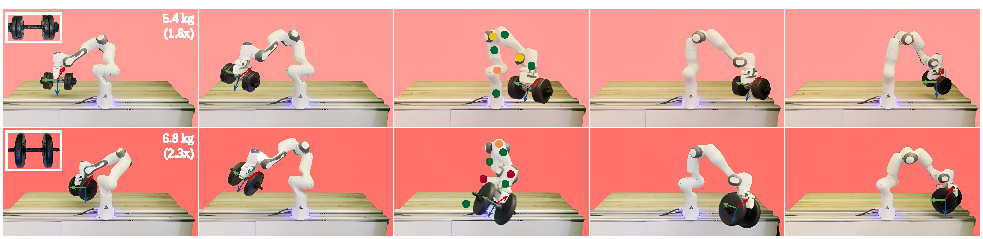
\includegraphics[width=\columnwidth]{graphics/vignew.pdf}
  \caption{Two qualitative motions of the robot carrying super-nominal payloads of \textcolor{pink}{$5.4$kg ($1.8\times$ nominal capacity)} and \textcolor{pastelred}{$6.8$kg ($2.3\times$ nominal capacity)} are shown. Colored dots indicate joint torques as a percentage of joint limits: \textcolor{green}{$0-20\%$}, \textcolor{midgreen}{$20-40\%$}, \textcolor{mid}{$40-60\%$}, \textcolor{midred}{$60-80\%$}, \textcolor{red}{$80-100\%$}. Joints 1, 3, and 5 exhibit higher torques, with joint 1 bearing the structural load of the arm and joints 3 and 5 positioning and orienting the payload.\vspace{-0.2in}}\label{fig:vignette}
\end{figure}
